
\section{Contribution 3: Platform : Human-Swarm Interaction}
ADD IMAGE SHOWING Parallel access to services.
\begin{figure}[htbp]
    \centerline{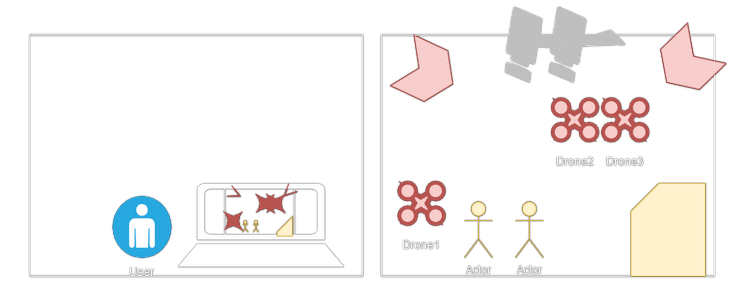
\includegraphics{images/setting.png}}
    \caption{ Our setup for controlling drones indoors around humans. }
    \label{fig}
    \end{figure}	



\subsection{Introduction}
In this section, we present our third contribution, which is the platform for human-swarm interaction. We present the setup and the software architecture that we have developed to control drones indoors around humans. We also present the results of the evaluation of the platform.

Our solution works on premise with a web-based interface to control the drones as it requires real-time computation. Both for drone control and human pose detection computation both have to be synchronized as both subjects are in the same environment. But the applications can be hosted on a cloud or other server allowing for remote control of the drones. This allows for a more flexible and scalable system.

\subsection{Platform for Human-Swarm Interaction}


Simulating drones in a virtual environment allows for the development of control algorithms without the need for physical drones. This is especially useful for testing new control strategies and algorithms in a safe and controlled environment. The platform provides a web-based interface for controlling the drones and visualizing their positions and orientations in real-time. The platform also provides a \gls{3D} visualization of the drones in the environment, allowing users to see the drones' positions and orientations in real-time. The platform is designed to be flexible and extensible, allowing for the addition of new features and functionalities as needed.
It acts as a monitoring tool for the platform. 
\begin{figure}[htbp]
    \centerline{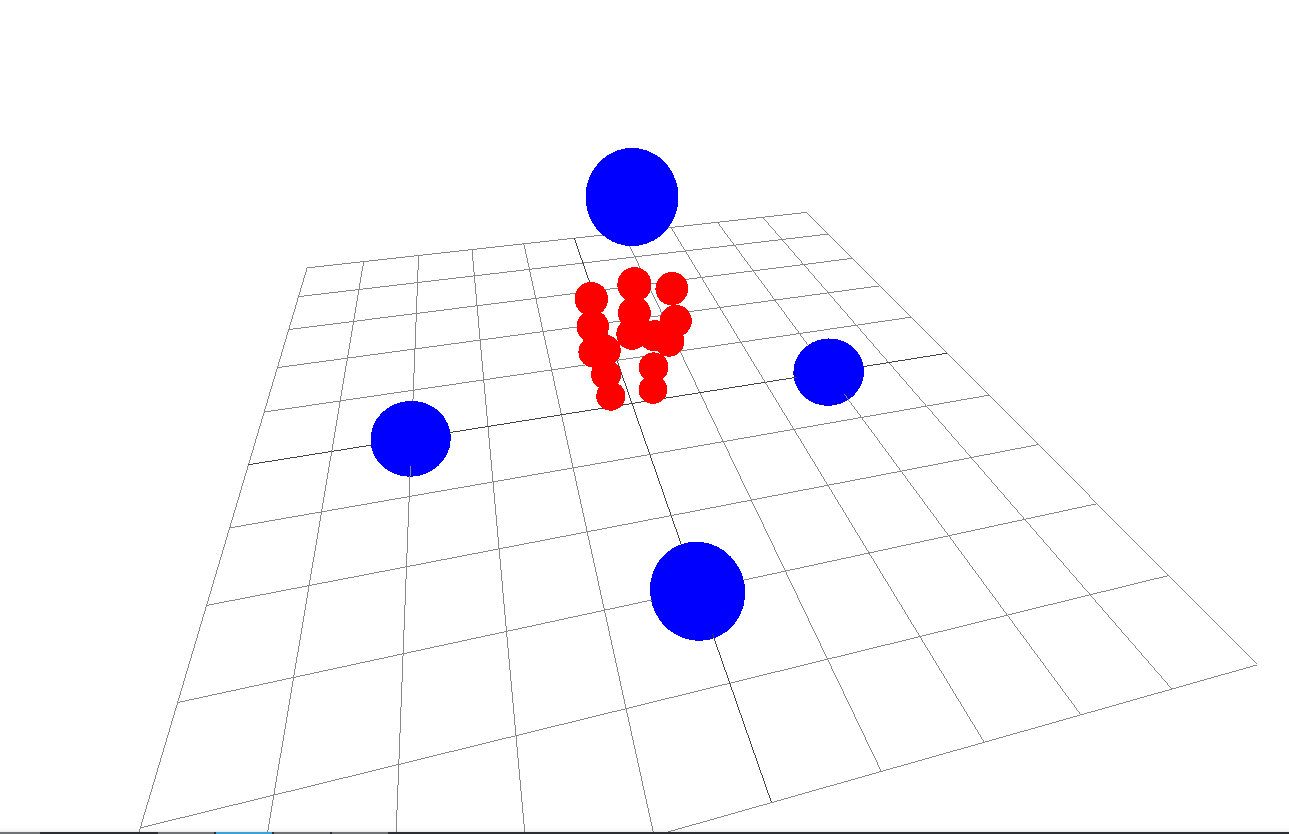
\includegraphics{images/image.png}}
    \caption{Shows the positions  of the elements of the platform through its web interface run for a few seconds.}
    \label{fig}
    \end{figure}

\begin{figure}[htbp]
    \centerline{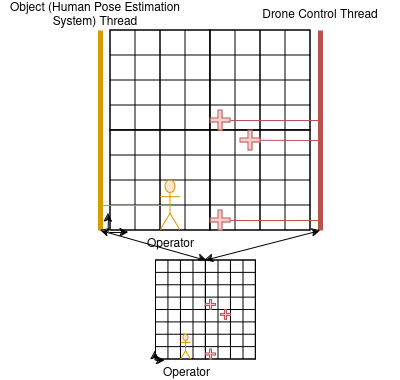
\includegraphics{images/ComboClient.png}}
    \caption{Shows the functionalities of the platform through its web interface and double threads. Above the realworld view and below the estimation after letting the system run for a few seconds.}
    \label{fig}
    \end{figure}
A user would then want to set speeds through his own app.
\subsection{Opportunitites}

As we have successfully built a usable platform with known people and subjects. We plan on testing it further and giving it to students to test further and develop on.
Students can access the platform and develop their own algorithms to control the drones and have them interact with them in real-time. This will allow students to experiment with different control strategies and learn about the challenges of controlling drones in indoor environments. Especially without having to work on the hardware part of the drones.

One student Maximilien Menesguen \cite{max} developed the famous boids \cite{reynolds1987boids} algorithm in Unity to make the drones follow a moving point in space using our UDP server, a work in progress. 
One of the main challenges in controlling drones indoors around humans is ensuring that the drones can avoid collisions with people and objects. The system continuously monitors the surroundings and adjusts the simulated drones' trajectories to avoid collisions.
it is based on the original boids algorithm. \cite{reynolds1987boids}. The boids algorithm is a simple and elegant model for simulating the flocking behavior of birds. It is based on three simple rules: separation, alignment, and cohesion. The separation rule ensures that the drones maintain a safe distance from each other, the alignment rule ensures that the drones move in the same direction, and the cohesion rule ensures that the drones stay together as a group. By following these rules, the drones can navigate the environment safely and efficiently.

The alignment rule is modified to take into account the position of the human operator so the drones interact more with the human. Thus we plan on seting the red Ball of the UAVs to be the user. This modification allows the drones to follow the human operator while maintaining a safe distance from them. The cohesion rule is also modified to ensure that the drones stay within a predefined area around the human operators. This modification would allow the drones to move around the human operator without straying too far from them.

We plan on adding the repulsion rule directly to the human operator and the drones. This rule would ensure that the drones maintain a safe distance from the human operator at all times. Adding the security layer to the platform is also a priority.

\begin{figure}[htbp]
    \centerline{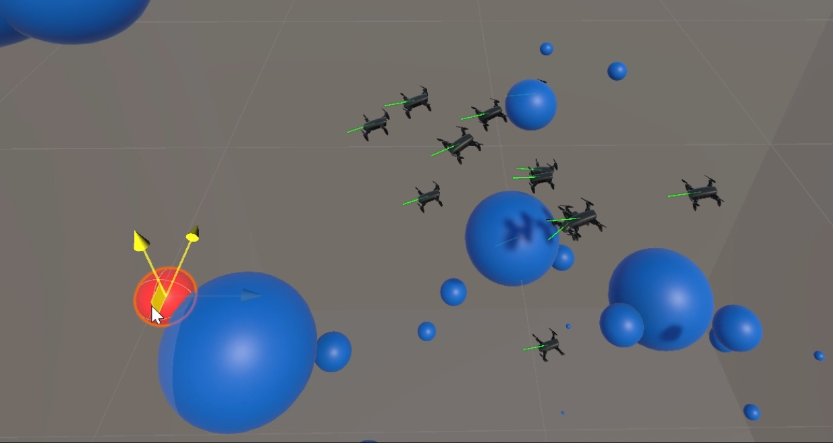
\includegraphics{images/dronesUnity.png}}
    \caption{ Drones following a moving point in space. }
    \label{fig}
    \end{figure}	


